\documentclass[14pt]{extreport}
\usepackage{gost}



\begin{document}
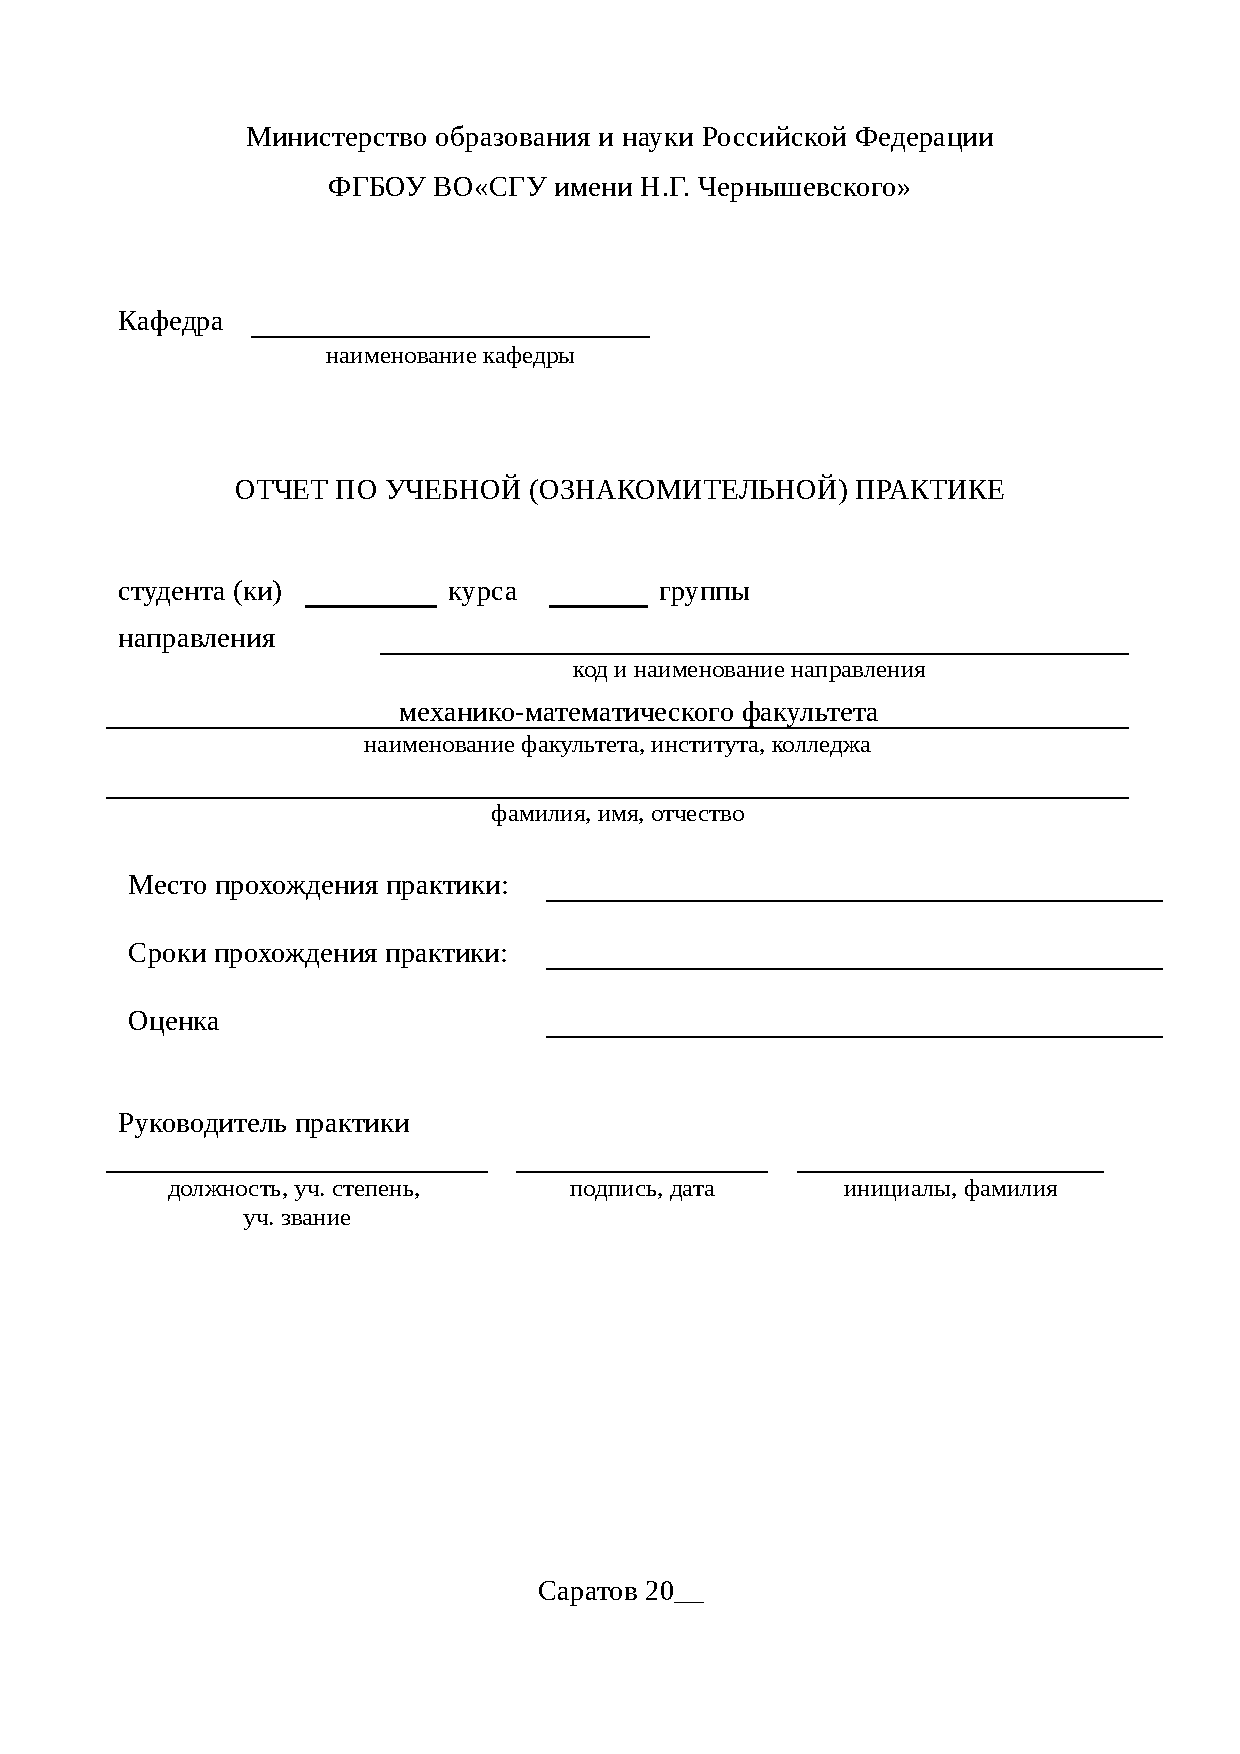
\includepdf[pages={1}]{titulOzPrac.pdf}


\tableofcontents

\intro

Ознакомительная практика является неотъемлемой частью учебного процесса. Студентам необходима подготовка к осознанному и углубленному изучению общепрофессиональных и специальных дисциплин и получение навыков самостоятельной практической работы по сбору фактического материала, составлению базы данных для различных исследований, анализа собранной информации.




\chapter{Множества. Действительные числа}

\section{Основные понятия}

Под множеством понимают совокупность (собрание, класс, семейство...) некоторых объектов, объединенных по какому-либо признаку.
Множество обозначается заглавными буквами, например $M$, $X$. Прописными латинскими буквами обозначаются элементы множеств, например $a$, $x$.
\begin{itemize}
\item $a \in M$ - элемент $a$ принадлежит множеству $M$;
\item $a \notin M$ - элемент $a$ не принадлежит множеству $M$;
\item $\exists$ - <<существует>>;
\item $\exists x \in M$ - существует $x$ из $M$;
\item $\forall$ - <<для любого>>, <<для всякого>>;
\item $a \wedge b$ - конъюнкция (<<и>>) - логическое умножение;
\item $a \vee b$  - дизъюнкция (<<или>>) - логическое сложение;
\item $\neg$ - <<не>> - логическое отрицание, например $\neg \forall x \in M$ - не для всех $x$ из $M$
\item $:$ - <<имеет место>>, <<такое что>>.
\end{itemize}



\section{Числовые множества. Множества действительных чисел}

Множества, элементами которых являются числа, называются \emph{числовыми}. Примерами числовых множеств являются:
\begin{itemize}
\item $N = \{1; 2; 3; ...; n; ...\}$ - множество натуральных чисел;
\item $Z_0 = \{0; 1; 2; ...; n; ...\}$ - множество целых неотрицательных чисел;
\item $Z = \{0; \pm 1; \pm 2; ...; \pm n; ...\}$ - множество целых чисел;
\item $Q = \{\frac mn : m \in Z, n \in N\}$ - множество рациональных чисел;
\item $R$ - множество действительных чисел.
\end{itemize} 

Действительные числа, не являющиеся рациональными, называются \emph{иррациональными}.



\section{Числовые промежутки. Окрестность точки}

Пусть $x_0$ - любое дейтвительное число (точка на числовой прямой). \emph{Окрестностью} точки $x_0$ называется любой интервал $(a; b)$, содержащий точку $x_0$. В частности, интервал $(x_0 - \varepsilon, x_0 + \varepsilon)$, где $\varepsilon > 0$, называется $\varepsilon$-окрестностью точки $x_0$. Число $x_0$ называется \emph{центром}, а число $\varepsilon$ - \emph{радиусом}.

\begin{figure}[H]
\centerline{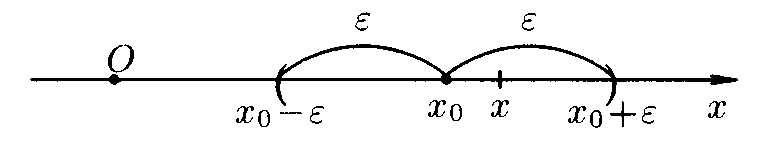
\includegraphics[width=1.0\linewidth]{pic1}}
\caption{Проверка точного решения}
\label{fig11}
\end{figure}

Если $x \in (x_0 - \varepsilon; x_0 + \varepsilon)$, то выполняется неравенство $x_0 - \varepsilon < x < x_0 + \varepsilon$, или, что то же, $|x - x_0| < \varepsilon$. Выполнение последнего неравенства означает попадание точки $x$ в $\varepsilon$-окрестность точки $x_0$ (см. рис. 1.1).






\chapter{Функция}


\section{Числовые функции. График функции}

1. $f(x)=3x^2$
\begin{figure}[H]
\centerline{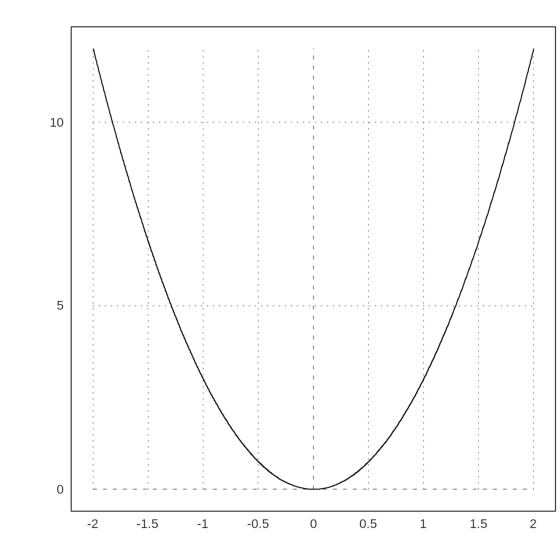
\includegraphics[width=1.0\linewidth]{gra-001}}
\caption{График функции - параболла}
\label{fig12}
\end{figure}

2. $f(x)=|x|$
\begin{figure}[H]
\centerline{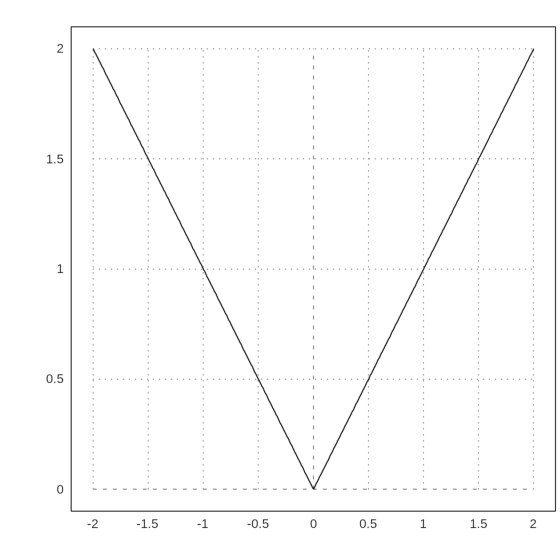
\includegraphics[width=1.0\linewidth]{gra-002}}
\caption{График функции - $f(x)=|x|$}
\label{fig13}
\end{figure}

\section{Обратная функция}

Найти функцию обратную для $y=3x+2$

Выразим $x$ через $y$, получаем: 
\begin{equation}
x = \frac{1}{3}y-\frac{2}{3} 
\end{equation}

Это и есть обратная функция, переставив буквы $x$ и $y$, будем писать: $y=\frac{1}{3}x-\frac{2}{3}$.

Таким образом, $y=3x+2$ и $y=\frac{1}{3}x-\frac{2}{3}$ - взаимно обратные функции.
\begin{figure}[H]
\centerline{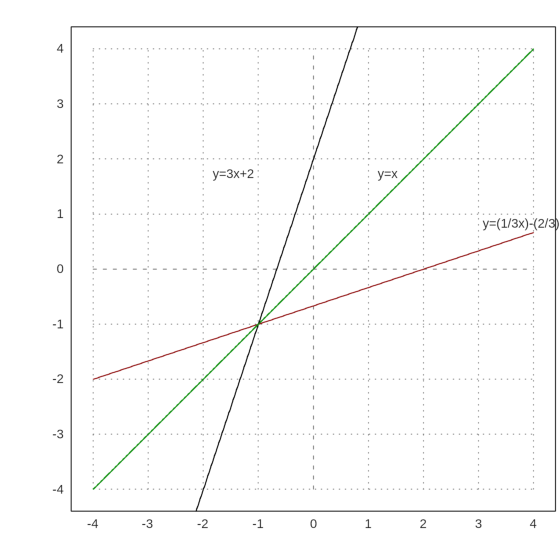
\includegraphics[width=1.0\linewidth]{gra-003}}
\caption{}
\label{fig14}
\end{figure}
 



\chapter{Последовательности}

\section{Числовая последовательность}

\section{Предел числовой последовательности}

\section{Предельный переход в неравенствах}

\section{Предел монотонной ограниченной последовательности. Число $e$. Натуральные логарифмы}



\chapter{Предел функции}

\section{Предел функции в точке}

\section{Односторонние пределы}

\section{Предел функции при $x\to\infty$}

\section{Бесконечно большая функция}



\chapter{Бесконечно малые функции}

\section{Определения и основные теоремы}

\section{Связь между функцией, ее пределом и бесконечно малой функцией}

\section{Основные теоремы о пределах}

\section{Признаки существования пределов}

\section{Первый замечательный предел}

\section{Второй замечательный предел}



\chapter{Эквивалентные бесконечно малые функции}

\section{Сравнение бесконечно малых функций}

\section{Эквивалентные беконечно малые и основные теоремы о них}

\section{Применение эквивиалентных бесконечно малых функций}



\chapter{Непрерывность функций}

\section{Непрерывность функции в точке}

\section{Непрерывность функции в интервале и на отрезке}

\section{Точки разрыва функции и их классификация}

\section{Основные теоремы о непрерывных функциях. Непрерывность элементарных функций}

\section{Свойства функций непрерывных на отрезке}



\chapter{Производная функции}


























\end{document}